\section{Actividad No 10 – Conjuntos} 
		


\begin{enumerate}[1.]
	\item El departamento de Recursos Humanos requiere un reporte de todos los departamentos que no contengan un empleado con el puesto ‘ST\_CLERK’. Utilizar el operador MINUS o EXCEPT para esta solicitud.
	\\
	\\select department\_id from employees
	\\where job\_id ='ST\_CLERK';

	\begin{center}
	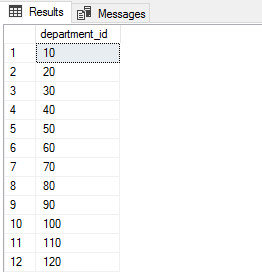
\includegraphics[width=5cm]{./Imagenes/ejercicio10-1} 
	\end{center}

	\item El departamento de Recursos Humanos requiere adicionalmente una lista de todos los pa\'ises que no tengan un departamento de la empresa localizado en ellos, mostrar el código del país y el nombre. Utilizar el operador MINUS o EXCEPT para realizar esta operaci\'on.
	\\
	\\select county\_id, country\_name from countries
	\\minus

	\begin{center}
	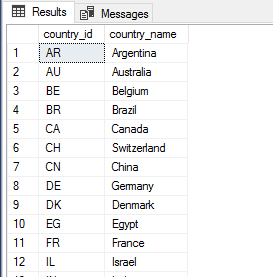
\includegraphics[width=5cm]{./Imagenes/ejercicio10-2} 
	\end{center}

	\item Se necesita una lista de puestos de los departamentos 10, 50 y 20, en ese orden, mostrar el c\'odigo del puesto y c\'odigo del departamento. Utilizar el operador UNION ALL.
	\\
	\\select distinct job\_id, department\_id from employees
	\\where (department\_id=10) 	
	\\union
	\\select distinct job\_id, department\_id from employees
	\\where (department\_id=50)
	\\union
	\\select distinct job\_id, department\_id from employees
	\\where  (department\_id=20);

	\begin{center}
	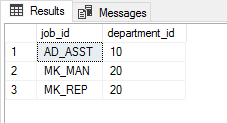
\includegraphics[width=5cm]{./Imagenes/ejercicio10-3} 
	\end{center}

	\item Crear un reporte que muestre que liste los c\'odigos de los empleados y los puestos de todos aquellos empleados que tienen el mismo puesto que en el momento en el que fueron contratados por la empresa, cambiaron de puestos y luego volvieron al puesto anterior. Utilizar el operador INTERSECT.
	\\
	\\select employee\_id, job\_id from employees
	\\intersect
	\\select distinct employee\_id, job\_id from job\_history;

	\begin{center}
	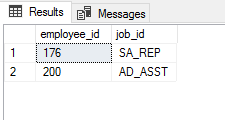
\includegraphics[width=5cm]{./Imagenes/ejercicio10-4} 
	\end{center}

	\item El departamento de Recursos Humanos requiere un reporte que muestre lo siguiente:

	\begin{itemize}
		\item Apellidos y c\'odigos de departamentos de todos los registros de la tabla empleados sin importar si pertenecen a uno o ningún departamento.
		\item C\'odigo de departamentos y nombres de departamentos de la tabla DEPARTAMENTOS inclusive si no existiese ningún empleado en ese departamento
	\end{itemize}
	Ambos requerimientos se deben mostrar en un mismo resultado. Utilizar el operador UNION ALL.
	\\
	\\select last\_name, department\_id, null from employees union select null, department\_id, department\_name from departments;

	\begin{center}
	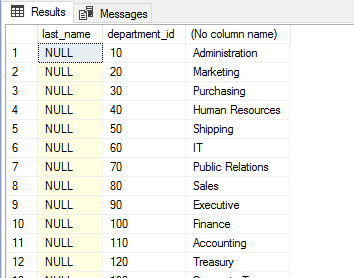
\includegraphics[width=5cm]{./Imagenes/ejercicio10-5} 
	\end{center}

\end{enumerate}